
%{{第五十五回}}{第五十五回}}

\chapter{辱亲女愚妾争闲气\hspace{.5em}欺幼主刁奴蓄险心}

{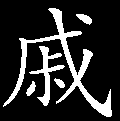
\includegraphics[width=3mm]{../Images/00005}  \kaishu 此回接上文,恰似黄钟大吕后,转出羽调商声,别有清凉滋味。}

且说元宵已过,只因当今以孝治天下,目下宫中有一位太妃欠安,故各嫔妃皆为之减膳谢妆,不独不能省亲,亦且将宴乐俱免。故荣府今岁元宵亦无灯谜之集。

刚将年事忙过,凤姐儿便小月了,在家一月,不能理事,天天两三个太医用药。凤姐儿自恃强壮,虽不出门,然筹画计算,想起什么事来,便命平儿去回王夫人,任人谏劝,他只不听。王夫人便觉失了膀臂,一人能有许多的精神?凡有了大事,自己主张;将家中琐碎之事,一应都暂令李纨协理。李纨是个尚德不尚才的,未免逞纵了下人。王夫人便命探春合同李纨裁处,只说过了一月,凤姐将息好了,仍交与他。谁知凤姐禀赋气血不足,兼年幼不知保养,平生争强斗智,心力更亏,故虽系小月,竟着实亏虚下来,一月之后,复添了下红之症。他虽不肯说出来,众人看他面目黄瘦,便知失于调养。王夫人只令他好生服药调养,不令他操心。他自己也怕成了大症,遗笑于人,便想偷空调养,恨不得一时复旧如常。谁知一直服药调养到八九月间,才渐渐的起复过来,下红也渐渐止了。此是后话。

如今且说目今王夫人见他如此,探春与李纨暂难谢事,园中人多,又恐失于照管,因又特请了宝钗来,托他各处小心,“老婆子们不中用,得空儿吃酒斗牌,白日里睡觉,夜里斗牌,我都知道的。凤丫头在外头,他们还有个惧怕,如今他们又该取便了。好孩子,你还是个妥当人,你兄弟妹妹们又小,我又没工夫,你替我辛苦两天,照看照看。凡有想不到的事,你来告诉我,别等老太太问出来,我没话回。那些人不好,你只管说。他们不听,你来回我。别弄出大事来才好。”宝钗听说只得答应了。

时届孟春,黛玉又犯了嗽疾。湘云亦因时气所感,亦卧病于蘅芜苑,一天医药不断。探春同李纨相住间隔,二人近日同事,不比往年,来往回话人等亦不便,故二人议定:每日早晨皆到园门口南边的三间小花厅上去会齐办事,吃过早饭于午错方回房。这三间厅原系预备省亲之时众执事太监起坐之处,故省亲之后也用不着了,每日只有婆子们上夜。如今天已和暖,不用十分修饰,只不过略略的铺陈了,便可他二人起坐。这厅上也有一匾,题着“辅仁谕德”四字,家下俗呼皆只叫议事厅儿。如今他二人每日卯正至此,午正方散。凡一应执事媳妇等来往回话者,络绎不绝。

众人先听见李纨独办,各各心中暗喜,以为李纨素日原是个厚道多恩无罚的,自然比凤姐儿好搪塞。便添了一个探春,也都想着不过是个未出闺阁的年轻小姐,且素日也最平和恬淡,因此都不在意,比凤姐儿前更懈怠了许多。只三四日后,几件事过手,渐觉探春精细处不让凤姐,只不过是言语安静,性情和顺而已。{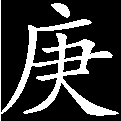
\includegraphics[width=3mm]{../Images/00004}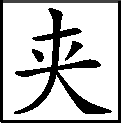
\includegraphics[width=3mm]{../Images/00012}\footnotesize \kaishu 这是小姐身份耳,阿凤未出阁想亦如此。}可巧连日有王公侯伯世袭官员十几处,皆系荣宁非亲即友或世交之家,或有升迁,或有黜降,或有婚丧红白等事,王夫人贺吊迎送,应酬不暇,前边更无人。他二人便一日皆在厅上起坐。宝钗便一日在上房监察,至王夫人回方散。每于夜间针线暇时,临寝之先,坐了小轿带领园中上夜人等各处巡察一次。他三人如此一理,更觉比凤姐儿当差时倒更谨慎了些。因而里外下人都暗中抱怨说:“刚刚的倒了一个‘巡海夜叉’,又添了三个‘镇山太岁’,越性连夜里偷着吃酒顽的工夫都没了。”

这日王夫人正是往锦乡侯府去赴席,李纨与探春早已梳洗,伺候出门去后,回至厅上坐了。刚吃茶时,只见吴新登的媳妇进来回说:“赵姨娘的兄弟赵国基昨日死了。昨日回过太太,太太说知道了,叫回姑娘奶奶来。”说毕,便垂手旁侍,再不言语。彼时来回话者不少,都打听他二人办事如何:若办得妥当,大家则安个畏惧之心;若少有嫌隙不当之处,不但不畏伏,出二门还要编出许多笑话来取笑。吴新登的媳妇心中已有主意,若是凤姐前,他便早已献勤说出许多主意,又查出许多旧例来任凤姐儿拣择施行。{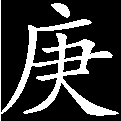
\includegraphics[width=3mm]{../Images/00004}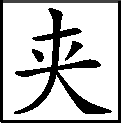
\includegraphics[width=3mm]{../Images/00012}\footnotesize \kaishu 可知虽有才干,亦必有羽翼方可。}如今他藐视李纨老实,探春是青年的姑娘,所以只说出这一句话来,试他二人有何主见。探春便问李纨。李纨想了一想,便道:“前儿袭人的妈死了,听见说赏银四十两。这也赏他四十两罢了。”吴新登家的听了,忙答应了是,接了对牌就走。探春道:“你且回来。”吴新登家的只得回来。探春道:“你且别支银子。我且问你:那几年老太太屋里的几位老姨奶奶,也有家里的也有外头的这两个分别。家里的若死了人是赏多少,外头的死了人是赏多少,你且说两个我们听听。”一问,吴新登家的便都忘了,忙陪笑回说:“这也不是什么大事,赏多少谁还敢争不成?”探春笑道:“这话胡闹。依我说,赏一百倒好。若不按例,别说你们笑话,明儿也难见你二奶奶。”吴新登家的笑道:“既这么说,我查旧账去,此时却记不得。”探春笑道:“你办事办老了的,还记不得,倒来难我们。你素日回你二奶奶也现查去?若有这道理,凤姐姐还不算利害,也就是算宽厚了!还不快找了来我瞧。再迟一日,不说你们粗心,反像我们没主意了。”吴新登家的满面通红,忙转身出来。众媳妇们都伸舌头,这里又回别的事。

一时,吴家的取了旧账来。探春看时,两个家里的赏过皆二十两,两个外头的皆赏过四十两。外还有两个外头的,一个赏过一百两,一个赏过六十两。这两笔底下皆有原故:一个是隔省迁父母之柩,外赏六十两;一个是现买葬地,外赏二十两。探春便递与李纨看了。探春便说:“给他二十两银子。把这账留下,我们细看看。”吴新登家的去了。

忽见赵姨娘进来,李纨探春忙让坐。赵姨娘开口便说道:“这屋里的人都踩下我的头去还罢了。姑娘你也想一想,该替我出气才是。”一面说,一面眼泪鼻涕哭起来。探春忙道:“姨娘这话说谁,我竟不解。谁踩姨娘的头?说出来我替姨娘出气。”赵姨娘道:“姑娘现踩我,我告诉谁!”探春听说,忙站起来,说道:“我并不敢。”李纨也站起来劝。

赵姨娘道:“你们请坐下,听我说。我这屋里熬油似的熬了这么大年纪,又有你和你兄弟,这会子连袭人都不如了,我还有什么脸?连你也没脸面,别说我了!”探春笑道:“原来为这个。我说我并不敢犯法违理。”一面便坐了,拿账翻与赵姨娘看,又念与他听,又说道:“这是祖宗手里旧规矩,人人都依着,偏我改了不成?也不但袭人,将来环儿收了外头的,自然也是同袭人一样。这原不是什么争大争小的事,讲不到有脸没脸的话上。他是太太的奴才,我是按着旧规矩办。说办的好,领祖宗的恩典、太太的恩典;若说办的不均,那是他糊涂不知福,也只好凭他抱怨去。太太连房子赏了人,我有什么有脸之处;一文不赏,我也没什么没脸之处。依我说,太太不在家,姨娘安静些养神罢了,何苦只要操心。太太满心疼我,因姨娘每每生事,几次寒心。我但凡是个男人,可以出得去,我必早走了,立一番事业,那时自有我一番道理。偏我是女孩儿家,一句多话也没有我乱说的。太太满心里都知道。如今因看重我,才叫我照管家务,还没有做一件好事,姨娘倒先来作践我。倘或太太知道了,怕我为难不叫我管,那才正经没脸,连姨娘也真没脸!”一面说,一面不禁滚下泪来。

赵姨娘没了别话答对,便说道:“太太疼你,你越发拉扯拉扯我们。你只顾讨太太的疼,就把我们忘了。”探春道:“我怎么忘了?叫我怎么拉扯?这也问你们各人,那一个主子不疼出力得用的人?那一个好人用人拉扯的?”李纨在旁只管劝说:“姨娘别生气。也怨不得姑娘,他满心里要拉扯,口里怎么说的出来。”探春忙道:“这大嫂子也糊涂了。我拉扯谁?谁家姑娘们拉扯奴才了?他们的好歹,你们该知道,与我什么相干。”赵姨娘气的问道:“谁叫你拉扯别人去了?你不当家我也不来问你。你如今现说一是一,说二是二。如今你舅舅死了,你多给了二三十两银子,难道太太就不依你?分明太太是好太太,都是你们尖酸刻薄,可惜太太有恩无处使。姑娘放心,这也使不着你的银子。明儿等出了阁,我还想你额外照看赵家呢。如今没有长羽毛,就忘了根本,只拣高枝儿飞去了!”

探春没听完,已气的脸白气噎,抽抽咽咽的一面哭,一面问道:“谁是我舅舅?我舅舅年下才升了九省检点,那里又跑出一个舅舅来?我倒素习按理尊敬,越发敬出这些亲戚来了。既这么说,每日环儿出去,为什么赵国基又站起来,又跟他上学?为什么不拿出舅舅的款来?何苦来,谁不知道我是姨娘养的,必要过两三个月寻出由头来,彻底来翻腾一阵,生怕人不知道,故意的表白表白。也不知谁给谁没脸?幸亏我还明白,但凡糊涂不知理的,早急了。”李纨急的只管劝,赵姨娘只管还唠叨。

忽听有人说:“二奶奶打发平姑娘说话来了。”赵姨娘听说,方把口止住。只见平儿进来,赵姨娘忙陪笑让坐,又忙问:“你奶奶好些?我正要瞧去,就只没得空儿。”李纨见平儿进来,因问他来做什么。平儿笑道:“奶奶说,赵姨奶奶的兄弟没了,恐怕奶奶和姑娘不知有旧例,若照常例,只得二十两。如今请姑娘裁夺着,再添些也使得。”探春早已拭去泪痕,忙说道:“又好好的添什么,谁又是二十四个月养下来的?不然也是那出兵放马背着主子逃出命来过的人不成?你主子真个倒巧,叫我开了例,他做好人,拿着太太不心疼的钱,乐的做人情。你告诉他,我不敢添减,混出主意。他添他施恩,等他好了出来,爱怎么添了去。”平儿一来时已明白了对半,今听这一番话,越发会意,见探春有怒色,便不敢以往日喜乐之时相待,只一边垂手默侍。

时值宝钗也从上房中来,探春等忙起身让坐。未及开言,又有一个媳妇进来回事。因探春才哭了,便有三四个小丫鬟捧了沐盆、巾帕、靶镜等物来。此时探春因盘膝坐在矮板榻上,那捧盆的丫鬟走至跟前,便双膝跪下,高捧沐盆;那两个小丫鬟,也都在旁屈膝捧着巾帕并靶镜脂粉之饰。平儿见待书不在这里,便忙上来与探春挽袖卸镯,又接过一条大手巾来,将探春面前衣襟掩了。探春方伸手向面盆中盥沐。那媳妇便回道:“回奶奶姑娘,家学里支环爷和兰哥儿的一年公费。”平儿先道:“你忙什么!你睁着眼看见姑娘洗脸,你不出去伺候着,先说话来。二奶奶跟前你也这么没眼色来着?姑娘虽然恩宽,我去回了二奶奶,只说你们眼里都没姑娘,你们都吃了亏,可别怨我。”唬的那个媳妇忙陪笑道:“我粗心了。”一面说,一面忙退出去。

探春一面匀脸,一面向平儿冷笑道:“你迟了一步,还有可笑的:连吴姐姐这么个办老了事的,也不查清楚了,就来混我们。幸亏我们问他,他竟有脸说忘了。我说他回你主子事也忘了再找去?我料着你那主子未必有耐性儿等他去找。”平儿忙笑道:“他有这一次,管包腿上的筋早折了两根。姑娘别信他们。那是他们瞅着大奶奶是个菩萨,姑娘又是个腼腆小姐,固然是托懒来混。”说着,又向门外说道:“你们只管撒野,等奶奶大安了,咱们再说。”门外的众媳妇都笑道:“姑娘,你是个最明白的人,俗语说,‘一人作罪一人当’,我们并不敢欺蔽小姐。如今小姐是娇客,若认真惹恼了,死无葬身之地。”平儿冷笑道:“你们明白就好了。”又陪笑向探春道:“姑娘知道二奶奶本来事多,那里照看的这些,保不住不忽略。俗语说‘旁观者清’,这几年姑娘冷眼看着,或有该添该减的去处二奶奶没行到,姑娘竟一添减,头一件于太太的事有益,第二件也不枉姑娘待我们奶奶的情义了。”话未说完,宝钗李纨皆笑道:“好丫头,真怨不得凤丫头偏疼他!本来无可添减的事,如今听你一说,倒要找出两件来斟酌斟酌,不辜负你这话。”探春笑道:“我一肚子气,没人煞性子,正要拿他奶奶出气去,偏他碰了来,说了这些话,叫我也没了主意了。”一面说,一面叫进方才那媳妇来问:“环爷和兰哥儿家学里这一年的银子,是做那一项用的?”那媳妇便回说:“一年学里吃点心或者买纸笔,每位有八两银子的使用。”探春道:“凡爷们的使用,都是各屋领了月钱的。环哥的是姨娘领二两,宝玉的是老太太屋里袭人领二两,兰哥儿的是大奶奶屋里领。怎么学里每人又多这八两?原来上学去的是为这八两银子!从今儿起,把这一项蠲了。平儿,回去告诉你奶奶,说我的话,把这一条务必免了。”平儿笑道:“早就该免。旧年奶奶原说要免的,因年下忙,就忘了。”那个媳妇只得答应着去了。就有大观园中媳妇捧了饭盒来。

待书素云早已抬过一张小饭桌来,平儿也忙着上菜。探春笑道:“你说完了话干你的去罢,在这里忙什么。”平儿笑道:“我原没事的。二奶奶打发了我来,一则说话,二则恐这里人不方便,原是叫我帮着妹妹们伏侍奶奶姑娘的。”探春因问:“宝姑娘的饭怎么不端来一处吃?”丫鬟们听说,忙出至檐外命媳妇去说:“宝姑娘如今在厅上一处吃,叫他们把饭送了这里来。”探春听说,便高声说道:“你别混支使人!那都是办大事的管家娘子们,你们支使他要饭要茶的,连个高低都不知道!平儿这里站着,你叫叫去。”

平儿忙答应了一声出来。那些媳妇们都忙悄悄的拉住笑道:“那里用姑娘去叫,我们已有人叫去了。”一面说,一面用手帕掸石矶上说:“姑娘站了半天乏了,这太阳影里且歇歇。”平儿便坐下。又有茶房里的两个婆子拿了个坐褥铺下,说:“石头冷,这是极干净的,姑娘将就坐一坐儿罢。”平儿忙陪笑道:“多谢。”一个又捧了一碗精致新茶出来,也悄悄笑说:“这不是我们的常用茶,原是伺候姑娘们的,姑娘且润一润罢。”平儿忙欠身接了,因指众媳妇悄悄说道:“你们太闹的不像了。他是个姑娘家,不肯发威动怒,这是他尊重,你们就藐视欺负他。果然招他动了大气,不过说他一个粗糙就完了,你们就现吃不了的亏。他撒个娇,太太也得让他一二分,二奶奶也不敢怎样。你们就这么大胆子小看他,可是鸡蛋往石头上碰。”众人都忙道:“我们何尝敢大胆了,都是赵姨奶奶闹的。”平儿也悄悄的说:“罢了,好奶奶们。‘墙倒众人推’,那赵姨奶奶原有些倒三不着两,有了事都就赖他。你们素日那眼里没人,心术利害,我这几年难道还不知道?二奶奶若是略差一点儿的,早被你们这些奶奶治倒了。饶这么着,得一点空儿,还要难他一难,好几次没落了你们的口声。众人都道他利害,你们都怕他,惟我知道他心里也就不算不怕你们呢。前儿我们还议论到这里,再不能依头顺尾,必有两场气生。那三姑娘虽是个姑娘,你们都横看了他。二奶奶这些大姑子小姑子里头,也就只单畏他五分。你们这会子倒不把他放在眼里了。”

正说着,只见秋纹走来。众媳妇忙赶着问好,又说:“姑娘也且歇一歇,里头摆饭呢。等撤下饭桌子,再回话去。”秋纹笑道:“我比不得你们,我那里等得。”说着便直要上厅去。平儿忙叫:“快回来。”秋纹回头见了平儿,笑道:“你又在这里充什么外围的防护?”一面回身便坐在平儿褥上。平儿悄问:“回什么?”秋纹道:“问一问宝玉的月银我们的月钱多早晚才领。”平儿道:“这什么大事。你快回去告诉袭人,说我的话,凭有什么事今儿都别回。若回一件,管驳一件;回一百件,管驳一百件。”秋纹听了,忙问:“这是为什么了?”平儿与众媳妇等都忙告诉他原故,又说:“正要找几件利害事与有体面的人开例作法子,镇压与众人作榜样呢。何苦你们先来碰在这钉子上。你这一去说了,他们若拿你们也作一二件榜样,又碍着老太太、太太;若不拿着你们作一二件,人家又说偏一个向一个,仗着老太太、太太威势的就怕,也不敢动,只拿着软的作鼻子头。你听听罢,二奶奶的事,他还要驳两件,才压的众人口声呢。”秋纹听了,伸舌笑道:“幸而平姐姐在这里,没的臊一鼻子灰。我赶早知会他们去。”说着,便起身走了。

接着宝钗的饭至,平儿忙进来伏侍。那时赵姨娘已去,三人在板床上吃饭。宝钗面南,探春面西,李纨面东。众媳妇皆在廊下静候,里头只有他们紧跟常侍的丫鬟伺候,别人一概不敢擅入。这些媳妇们都悄悄的议论说:“大家省事罢,别安着没良心的主意。连吴大娘才都讨了没意思,咱们又是什么有脸的。”他们一边悄议,等饭完回事。只觉里面鸦雀无声,并不闻碗箸之声。一时只见一个丫鬟将帘栊高揭,又有两个将桌抬出。茶房内早有三个丫头捧着三沐盆水,见饭桌已出,三人便进去了。一回又捧出沐盆并漱盂来,方有待书、素云、莺儿三个,每人用茶盘捧了三盖碗茶进去。一时等他三人出来,待书命小丫头子:“好生伺候着,我们吃饭来换你们,别又偷坐着去。”众媳妇们方慢慢的一个一个的安分回事,不敢如先前轻慢疏忽了。

探春气方渐平,因向平儿道:“我有一件大事,早要和你奶奶商议,如今可巧想起来。你吃了饭快来。宝姑娘也在这里,咱们四个人商议了,再细细的问你奶奶可行可止。”平儿答应回去。

凤姐因问为何去了这一日,平儿便笑着将方才的原故细细说与他听了。凤姐儿笑道:“好,好,好,好个三姑娘!我说他不错。只可惜他命薄,没托生在太太肚里。”平儿笑道:“奶奶也说糊涂话了。他便不是太太养的,难道谁敢小看他,不与别的一样看了?”凤姐儿叹道:“你那里知道,虽然庶出一样,女儿却比不得男人,将来攀亲时,如今有一种轻狂人,先要打听姑娘是正出是庶出,多有为庶出不要的。殊不知别说庶出,便是我们的丫头,比人家的小姐还强呢。将来不知那个没造化的挑庶正误了事呢,也不知那个有造化的不挑庶正的得了去。”说着,又向平儿笑道:“你知道,我这几年生了多少省俭的法子,一家子大约也没个不背地里恨我的。我如今也是骑上老虎了。虽然看破些,无奈一时也难宽放;二则家里出去的多,进来的少。凡百大小事仍是照着老祖宗手里的规矩,却一年进的产业又不及先时。多省俭了,外人又笑话,老太太、太太也受委屈,家下人也抱怨刻薄;若不趁早儿料理省俭之计,再几年就都赔尽了。”

平儿道:“可不是这话!将来还有三四位姑娘,还有两三个小爷,一位老太太,这几件大事未完呢。”凤姐儿笑道:“我也虑到这里,倒也够了:宝玉和林妹妹他两个一娶一嫁,可以使不着官中的钱,老太太自有梯己拿出来。二姑娘是大老爷那边的,也不算。剩下三四个,满破着每人花上一万银子。环哥娶亲有限,花上三千两银子,不拘那里省一抿子也就够了。老太太事出来,一应都是全了的,不过零星杂项,便费也满破三五千两。如今再俭省些,陆续也就够了。只怕如今平空又生出一两件事来,可就了不得了。------咱们且别虑后事,你且吃了饭,快听他商议什么。这正碰了我的机会,我正愁没个膀臂。虽有个宝玉,他又不是这里头的货,纵收伏了他也不中用。大奶奶是个佛爷,也不中用。二姑娘更不中用,亦且不是这屋里的人。四姑娘小呢。兰小子更小。环儿更是个燎毛的小冻猫子,只等有热灶火坑让他钻去罢。真真一个娘肚子里跑出这样天悬地隔的两个人来,我想到这里就不伏。再者林丫头和宝姑娘他两个倒好,偏又都是亲戚,又不好管咱家务事。况且一个是美人灯儿,风吹吹就坏了;一个是拿定了主意,‘不干己事不张口,一问摇头三不知’,也难十分去问他。倒只剩了三姑娘一个,心里嘴里都也来的,又是咱家的正人,太太又疼他,虽然面上淡淡的,皆因是赵姨娘那老东西闹的,心里却是和宝玉一样呢。比不得环儿,实在令人难疼,要依我的性早撵出去了。如今他既有这主意,正该和他协同,大家做个膀臂,{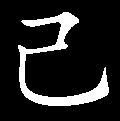
\includegraphics[width=3mm]{../Images/00003}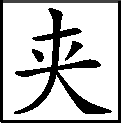
\includegraphics[width=3mm]{../Images/00012}\footnotesize \kaishu 阿凤有才处全在择人,收纳膀臂羽翼,并非一味倚才自恃者可知。这方是大才。}我也不孤不独了。按正理,天理良心上论,咱们有他这个人帮着,咱们也省些心,于太太的事也有些益。若按私心藏奸上论,我也太行毒了,也该抽头退步。回头看看了,再要穷追苦克,人恨极了,暗地里笑里藏刀,咱们两个才四个眼睛、两个心,一时不防,倒弄坏了。趁着紧溜之中,他出头一料理,众人就把往日咱们的恨暂可解了。还有一件,我虽知你极明白,恐怕你心里挽不过来,如今嘱咐你:他虽是姑娘家,心里却事事明白,不过是言语谨慎;他又比我知书识字,更厉害一层了。如今俗语‘擒贼必先擒王’,他如今要作法开端,一定是先拿我开端。倘或他要驳我的事,你可别分辩,你只越恭敬,越说驳的是才好。千万别想着怕我没脸,和他一犟,就不好了。”

平儿不等说完,便笑道:“你太把人看糊涂了。我才已经行在先,这会子又反嘱咐我。”凤姐儿笑道:“我是恐怕你心里眼里只有了我,一概没有别人之故,不得不嘱咐。既已行在先,更比我明白了。你又急了,满口里‘你’‘我’起来。”平儿道:“偏说‘你’!你不依,这不是嘴巴子,再打一顿。难道这脸上还没尝过的不成!”凤姐儿笑道:“你这小蹄子,要掂多少过子才罢。看我病的这样,还来怄我。过来坐下,横竖没人来,咱们一处吃饭是正经。”

说着,丰儿等三四个小丫头子进来放小炕桌。凤姐只吃燕窝粥,两碟子精致小菜,每日分例菜已暂减去。丰儿便将平儿的四样分例菜端至桌上,与平儿盛了饭来。平儿屈一膝于炕沿之上,半身犹立于炕下,陪凤姐儿吃了饭,{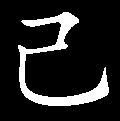
\includegraphics[width=3mm]{../Images/00003}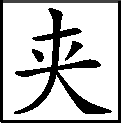
\includegraphics[width=3mm]{../Images/00012}\footnotesize \kaishu 凤姐之才又在能买邀人心。}伏侍漱盥。漱毕,嘱咐了丰儿些话,方往探春处来。只见院中寂静,人已散出。要知端的------

{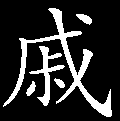
\includegraphics[width=3mm]{../Images/00005}  \kaishu 总评:噫!事亦难矣哉!探春以姑娘之尊,以贾母之爱,以王夫人之付托,以凤姐之未谢事,暂代数月,而奸奴蜂起,内外欺侮,锱铢小事,突动风波,不亦难乎!以凤姐之聪明,以凤姐之才力,以凤姐之权术,以凤姐之贵宠,以凤姐之日夜焦劳,百般弥缝,犹不免骑虎难下,为移祸东吴之计,不亦难乎!况聪明才力不及凤姐,权术贵宠不及凤姐,焦劳弥缝不及凤姐,又无贾母之爱,姑娘之尊,太太之付托,而欲左支右吾,撑前达后,不更难乎!士方有志作一番事业,每读至此,不禁为之投书以起,三复流连而欲泣也!}
